This section addresses the work progress within the ME. Refer to Sean Keene's thesis to get how the system is set up. This document, however, addresses an issue that is related to GridAPPS-D flexibility. 

\subsection{Problem Statement}

\begin{figure}[htp!]
    \centering
    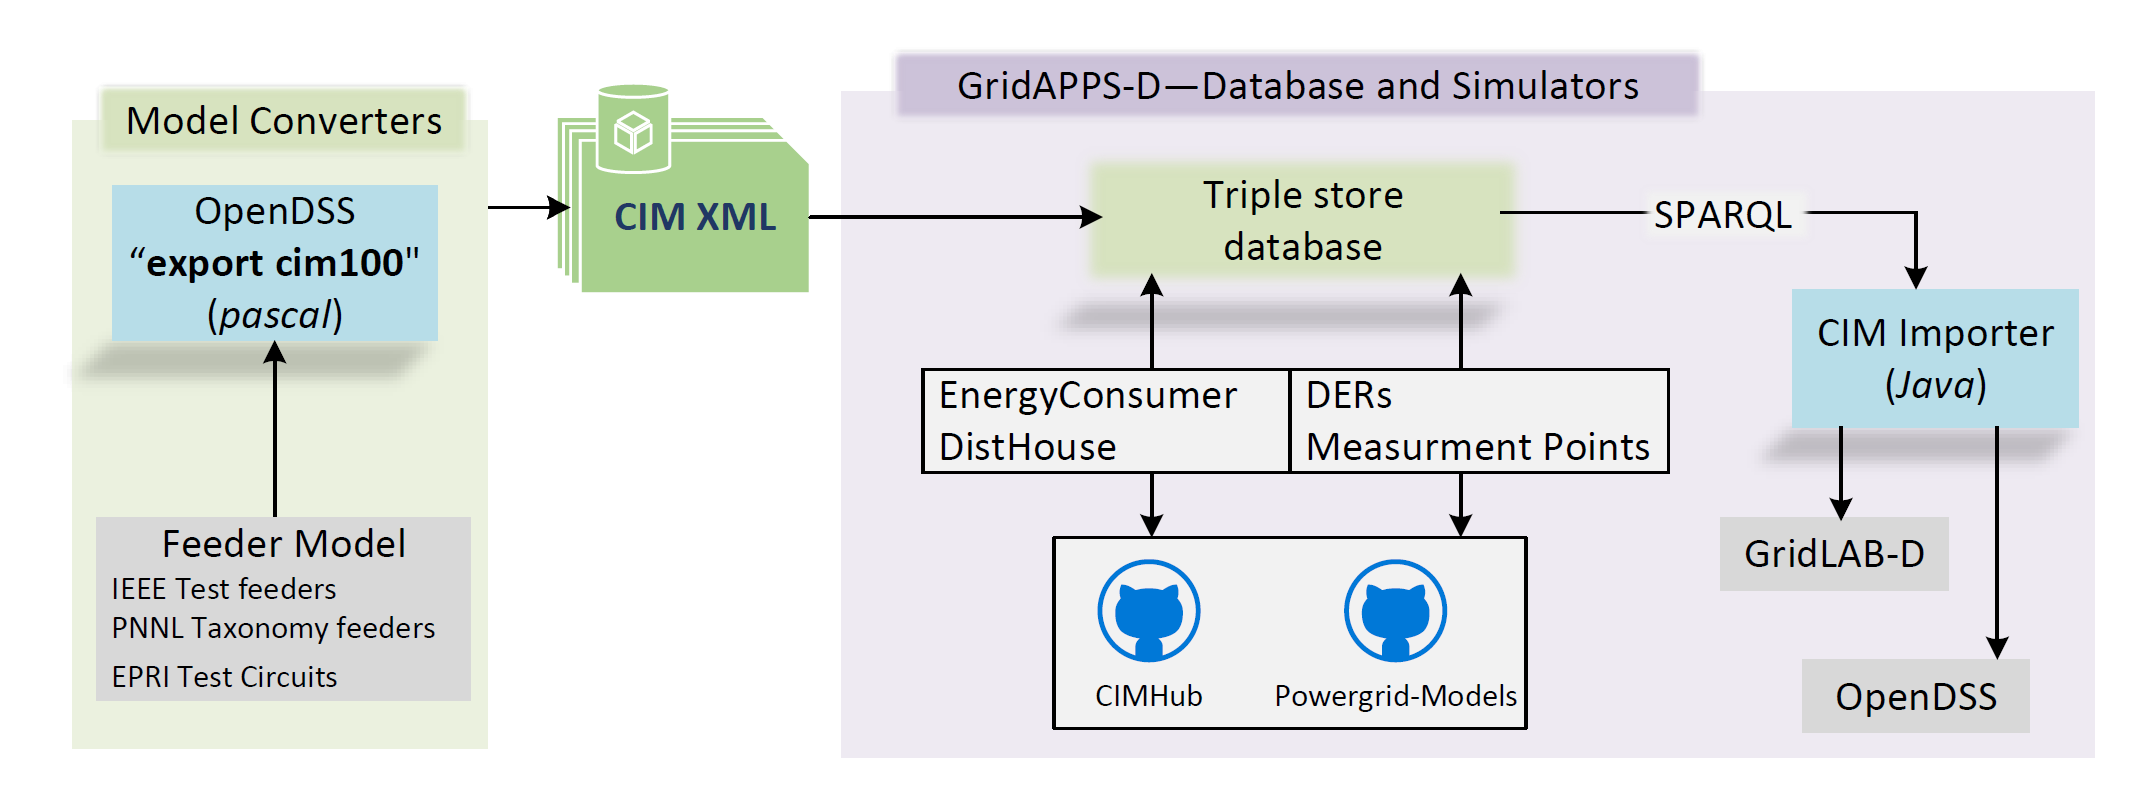
\includegraphics[width=0.7\columnwidth]{Pictures/model_conversion.png}
    \caption{GridAPPS-D Model Conversion}
    \label{fig:me_gridappsd}
\end{figure}

As shown in Figure~\ref{fig:me_gridappsd}, GridAPPS-D takes an input file (IEEE Test Feeders, PNNL Taxonomy Feeders, or EPRI Test Circuits) as a \textbf{dss} format. Within each \textbf{dss} file,
``export cim100'' command is used to export an XML version of the \textbf{dss} file. The XML file is then stored in the Triple Store database so it can be adjusted as needed. 


Over the years, the PowerLab team has been extensively working with GridLAB-D. The PowerLab team has developed several \textbf{glm} scripts to implement studies and cases. Many of these studies are slightly or non-GridAPPS-D-related. 
The time has come to merge many of these studies within the Modelling Environment (ME). This Section is meant to walk through the progress of implementing scripts that convert \textbf{glm} files to \textbf{dss}.

\subsection{Objectives}
\begin{itemize}
    \item Convert \textbf{glm} files to \textbf{Common Information Model (CIM)}.
    \item Insert the appropriate loads in the specified \textbf{glm} file using GridAPPS-D.
    \item Develop communication between entities and demand response capabilities.
\end{itemize}

\subsection{Tools to be Used}

\begin{itemize}
    \item To convert from GridLAB-D to OpenDSS, I used \href{https://github.com/NREL/ditto}{Ditto-CLI}
    \item To edit the \textbf{glm} files, I used \href{https://github.com/NREL/glm}{glm} module in Python.
    \item To convert from \textbf{dss} to \textbf{CIM}, I used \href{https://cimhub.readthedocs.io/en/latest/Tutorial.html#ieee-123-bus-base-case}{CIMhub}
\end{itemize}

\subsection{Processing Steps}

\begin{figure}[htp!]
    \centering
    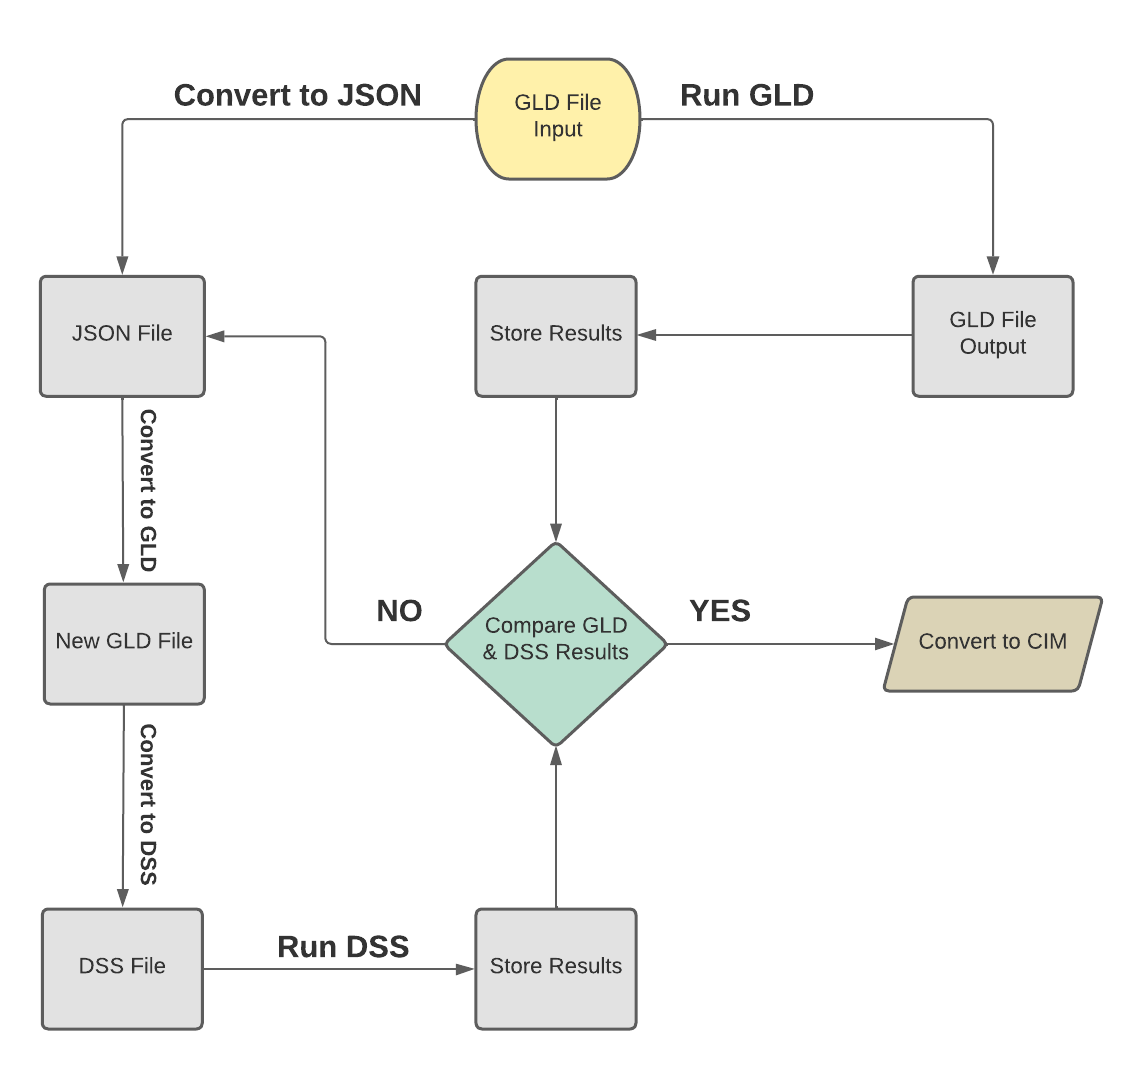
\includegraphics[width=0.7\columnwidth]{Pictures/glm_conversion_tool.png}
    \caption{File Conversion Processing Chart}
    \label{fig:me_conversion}
\end{figure}

\subsubsection{Step 1: Edit \textbf{glm} Files}

GridLAB-D and OpenDSS are different software packages and, therefore, they are not expected to have the same models. To find out which GridLAB-D objects are compatible with OpenDSS models, I went through test files 
within \href{https://github.com/NREL/ditto}{Ditto-CLI}. The \href{run: /home/deras/Desktop/Midrar_work/ditto/tests/data/small_cases/gridlabd/ieee_4node/node.glm}{Node.glm} is a \textbf{glm} file that can be easily 
converted to \textbf{dss} without errors. The content of this file is compared with the \textbf{glm} that I developed to ensure a smooth and accurate transition between GridLAB-D and OpenDSS.